% Appendix: the additive case of the fixed-menu bound (thm:B) (best fixed menu = 5/6).  Requires \appendix before inclusion.
\section{The additive case: the best fixed menu is exactly $5/6$}
\label{app:sd}

\paragraph{Upper bound.} At $\varepsilon=0$ Theorem~\ref{thm:B} holds in a stronger form: let
$M(x,y)=\lambda A(x)+(1-\lambda)B(y)$, where $A$ depends only on agent~1's report and $B$ only on
agent~2's (every swap-dictatorial mechanism, with any menus, is of this form); then $M$ is at most
$5/6$-competitive. \emph{Proof.} Let $a(x)$ be agent~1's expected share of item~1 minus item~2 under $A(x)$, and $b(y)$ likewise
under $B(y)$; both lie in $[-1,1]$. With additive valuations an allocation with net share $d$
for agent~1 yields welfare $1+(x-y)d$, so $W(x,y)=1+(x-y)[\lambda a(x)+(1-\lambda)b(y)]$. On the four
profiles $(\tfrac12,0),(1,\tfrac12),(0,\tfrac12),(\tfrac12,1)$, each with first-best welfare $\tfrac32$,
the terms of the middle type cancel and
\[
\textstyle\sum W=4+\tfrac12\lambda\,[a(1)-a(0)]+\tfrac12(1-\lambda)\,[b(1)-b(0)]\le5 ,
\]
so some profile has $W\le\tfrac54=\tfrac56\cdot\tfrac32$. \qed

\paragraph{Attainment: reduction to one function.} Consider a symmetric swap-dictatorial mechanism in which
the dictator of type $x$ receives $(m_1(x),m_2(x))$ and write $d(x)=m_1(x)-m_2(x)$. If agent~1 is
the dictator, welfare is $xm_1+(1-x)m_2+y(1-m_1)+(1-y)(1-m_2)=1+(x-y)d(x)$; if agent~2 (type $y$) is,
it is $1+(y-x)d(y)$. Averaging, for $x>y$,
\[
W(x,y)=1+\tfrac12(x-y)\,[d(x)-d(y)],\qquad \mathrm{OPT}(x,y)=1+(x-y),
\]
and with $s=x-y$, $W/\mathrm{OPT}\ge\tfrac56$ is equivalent to $d(x)-d(y)\ge h(s):=\tfrac53-\tfrac1{3s}$.
The constraint is vacuous for $s\le\tfrac15$.

\paragraph{Incentive compatibility.} A type-$x$ dictator's utility from item $(m_1,m_2)$ is
$m_2+x\,(m_1-m_2)$, affine in $x$. A choice function is implementable by a fixed menu with
truthful reporting if and only if $d$ is non-decreasing and the dictator's utility satisfies the
envelope formula $U(x)=U(0)+\int_0^x d$; the shares are then $m_2=U-xd$ and $m_1=U+(1-x)d$
(the standard single-crossing characterisation, as for Myerson's lemma). The menu is the set of
chosen items.

\paragraph{The steepest admissible $d$.} Let $D(x)$ be the supremum, over chains
$0=x_0<x_1<\dots<x_k=x$, of $\sum_i h^+(x_i-x_{i-1})$. Extending a chain to $y$ by one step shows
$D(x)\ge D(y)+h^+(x-y)$ for $x>y$, so $D$ is non-decreasing and satisfies the constraint. Because
$h$ is concave, for a fixed number $k$ of steps equal gaps are optimal (Jensen), so
\[
D(x)=\max_k\big[k\,h(x/k)\big]^+=\max_k\Big[\frac{5k}{3}-\frac{k^2}{3x}\Big]^+=
\begin{cases}0,& x\le\tfrac15,\\ \tfrac53-\tfrac1{3x},&\tfrac15\le x\le\tfrac35,\\ \tfrac{10}3-\tfrac4{3x},&\tfrac35\le x\le1,\end{cases}
\]
and $D(1)=\max_k k(5-k)/3=2$, attained at $k=2$ and $k=3$.

\paragraph{Symmetrisation.} Set $d(x)=\tfrac12[D(x)-D(1-x)]$. It is non-decreasing, $d(0)=-1$,
$d(1)=1$, and for $x>y$
\[
d(x)-d(y)=\tfrac12\big[D(x)-D(y)\big]+\tfrac12\big[D(1-y)-D(1-x)\big]\ge\tfrac12h(x-y)+\tfrac12h(x-y)=h(x-y),
\]
since $(1-y)-(1-x)=x-y$. With $U(0)=1$ (type $0$ takes item~2 in full) the envelope shares satisfy
$m_1(0)=0$, $m_2(0)=1$, $m_1(1)=1$, $m_2(1)=0$, and $0\le m_1,m_2\le1$ throughout; we verified the
last property numerically on a grid of $2\cdot10^5$ types (the shares touch the boundary only at
$x\in\{0,1\}$). The induced mechanism is therefore strategy-proof and $5/6$-competitive, and by
the upper bound above no swap-dictatorial mechanism does better. \qed

\paragraph{Discretisation.} A finite menu of $n$ items taken from this curve gives up a little,
because types between items choose a neighbouring one. Evaluating the ratio of such a menu
exactly on the continuum (the ratio is linear-fractional on each piece of a finite partition of
the type square, so its minimum is at a vertex) gives $0.83258$, $0.83315$ and $0.83328$ for
$n=501$, $2001$ and $8001$.

\begin{figure}[H]\centering
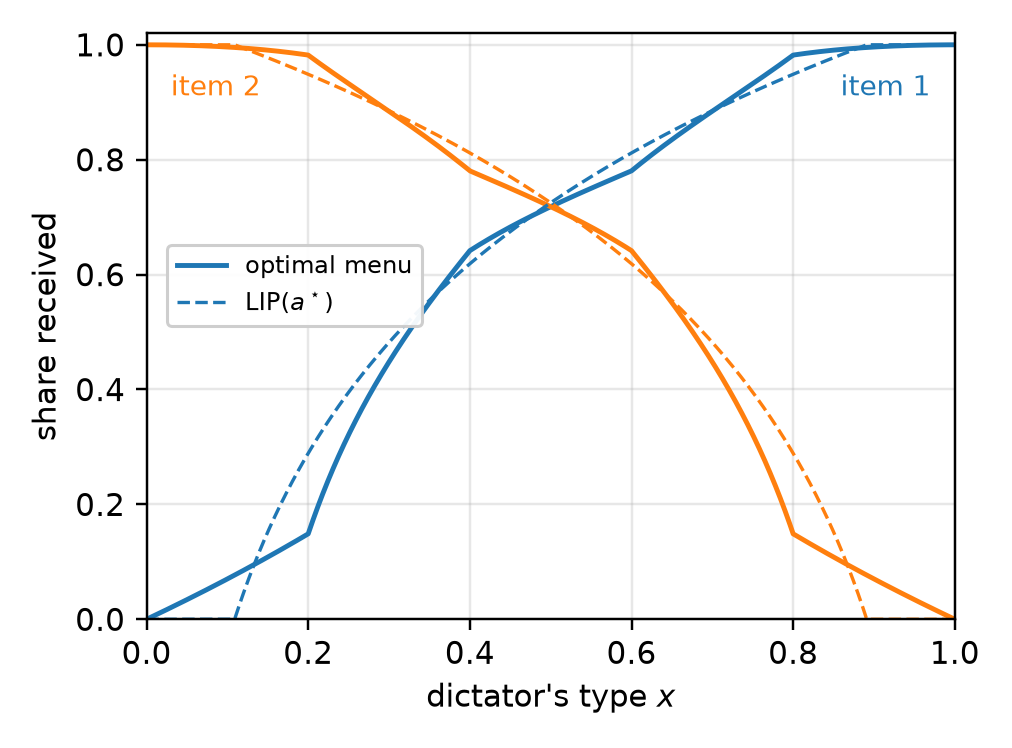
\includegraphics[width=0.55\linewidth]{figures/02_optimal_menu.png}
\caption{What a dictator of type $x$ receives under the $5/6$-competitive menu constructed above
(solid) and under LIP($a^\star$) (dashed); blue: item~1, orange: item~2. At the balanced type the
two nearly coincide; the optimal menu differs mainly near the extremes, where it still gives a
lopsided dictator a little of her less-preferred item.}
\label{fig:optimal_menu}
\end{figure}
